% maskera whitepaper. Compile: node scripts/build-whitepaper.mjs (tectonic).
% Output ships as apps/demo/public/whitepaper.pdf -> maskera.dev/whitepaper.pdf
% Numbers are a dated snapshot; docs/BENCHMARKS.md is always canonical.
\documentclass[10pt,a4paper]{article}

\usepackage[T1]{fontenc}
\usepackage{lmodern}
\usepackage{microtype}
\usepackage[margin=32mm,top=28mm,bottom=26mm]{geometry}
\usepackage{amssymb}
\usepackage{booktabs}
\usepackage{float}
\usepackage{array}
\usepackage{tikz}
\usetikzlibrary{positioning,arrows.meta}
\usepackage[hidelinks]{hyperref}
\usepackage{url}
\usepackage{parskip}
\setlength{\parskip}{0.34\baselineskip}
\setlength{\emergencystretch}{1em}

\newcommand{\pkg}[1]{\texttt{#1}}

\title{\textbf{Client-Side Redaction of Swedish\\Personally Identifiable Information}\\[0.6em]
\large\textmd{maskera: deterministic rules and a 43\,MB on-device NER model\\that mask PII before text reaches an LLM, a log, or analytics}}
\author{Joel H\"agvall\\[0.2em]
\normalsize\href{https://maskera.dev}{\texttt{maskera.dev}} \quad
\normalsize\href{https://github.com/joelhagvall/maskera}{\texttt{github.com/joelhagvall/maskera}}}
\date{August 10, 2026 \quad\textperiodcentered\quad Whitepaper v1.18}

\begin{document}
\maketitle

\begin{abstract}
\noindent maskera is an open-source (MIT) library that redacts personally
identifiable information in Swedish text locally, in the browser or in the
caller's own server process, before text is sent anywhere. Structured identifiers (personnummer,
organisation numbers, phone numbers, bank account references, and others) are
caught by deterministic, format-aware rules with selective checksums. Names, places,
organisations, and street addresses in free text are caught by a purpose-built
Swedish NER model of 43\,MB, small enough to run where the text already is,
including inside a browser tab. The input text never leaves the caller's
environment, the packages collect no telemetry, and the mapping that restores
masked values is held locally by the caller. In the default setup the browser
downloads the static assets once from a public host; self-hosting those
assets makes zero external requests. Measured on a small external Swedish gold set, the
pipeline flagged 98\% of PII entities and achieved the highest typed $F_1$
among the public Swedish NER models tested, at less than a tenth of their size. maskera is a
data-minimisation and data-protection-by-design tool, not a compliance
guarantee; this document reports method and limitations with the same candour
as the results. Intended readers: data protection officers, security teams,
architects, and legal reviewers.
\end{abstract}

\section{The problem: free text leaks PII}

Swedish organisations now send user-generated text to more external systems
than ever: large language models behind third-party APIs (frequently hosted
outside the EU/EEA), log platforms, analytics pipelines, and support tooling.
That text is largely free-form, and free-form text carries personal data:
customers type their personnummer into chat windows, case workers mention
names and home addresses in ticket notes, patients describe their situation
with full identities attached.

Every such flow is a processing operation under data-protection law. Where the
recipient is a third-party vendor, questions of processing agreements and
third-country transfers follow, and every system that stores the raw text
widens the incident surface. The simplest way to reduce all of these risks at
once is to not send the personal data at all.

The established technical countermeasures share two weaknesses. Server-side
DLP services and redaction proxies only see the text \emph{after} it has left
the client, and they are themselves one more system processing raw personal
data. The publicly available Swedish NER models, for their part, are on the
order of 500\,MB; they require a dedicated inference service with a GPU or a
strong CPU, which in practice again means a new system that sees the raw text.

maskera takes the opposite approach: redact the text \emph{where it already
is}, in the browser before a form is submitted, or inside the caller's own
server process before the outbound API call. No new data recipient is
introduced.

\section{Architecture: two layers, rules first}

\begin{figure}[h]
\centering
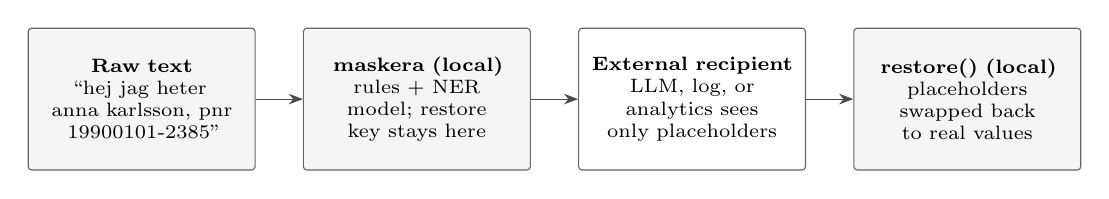
\begin{tikzpicture}[
  node distance=6mm,
  box/.style={draw=black!60, rounded corners=1.2pt, align=center,
              font=\scriptsize, inner sep=4pt, text width=26mm,
              minimum height=18mm},
  arr/.style={-{Stealth[length=1.8mm]}, black!70}
]
\node[box, fill=black!4] (raw) {\textbf{Raw text}\\``hej jag heter anna karlsson, pnr 19900101-2385''};
\node[box, fill=black!4, right=of raw] (mask) {\textbf{maskera (local)}\\rules + NER model; restore key stays here};
\node[box, right=of mask] (ext) {\textbf{External recipient}\\LLM, log, or analytics sees only placeholders};
\node[box, fill=black!4, right=of ext] (res) {\textbf{restore() (local)}\\placeholders swapped back to real values};
\draw[arr] (raw) -- (mask);
\draw[arr] (mask) -- (ext);
\draw[arr] (ext) -- (res);
\end{tikzpicture}
\end{figure}

The redaction flow is: raw text $\rightarrow$ \pkg{redact()} $\rightarrow$
masked text with placeholders $\rightarrow$ LLM / log / analytics
$\rightarrow$ \pkg{restore()} locally. The external recipient only ever sees
placeholders such as \texttt{[NAMN\_1]} and \texttt{[PERSONNUMMER\_1]};
shaded boxes run inside the caller's environment. Restoration is optional:
in many logging and analytics flows it is never performed, and the
placeholders are the final stored form.

\begin{figure}[h]
\centering
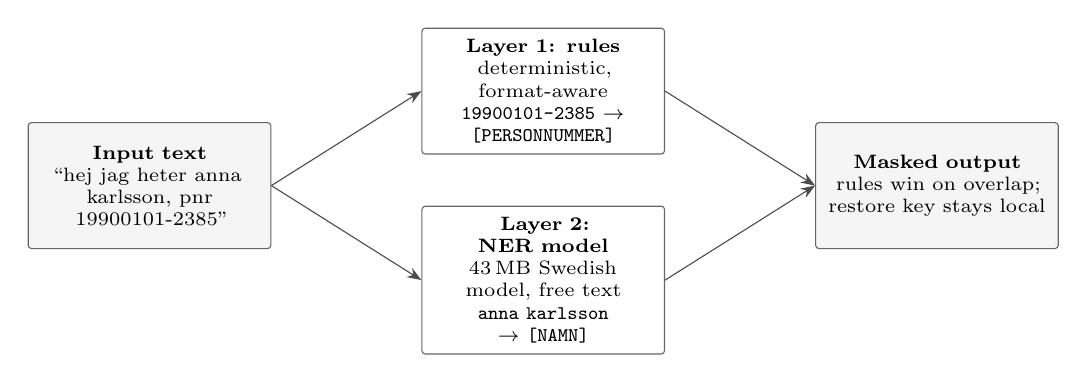
\begin{tikzpicture}[
  box/.style={draw=black!60, rounded corners=1.2pt, align=center,
              font=\scriptsize, inner sep=4pt, text width=28mm},
  arr/.style={-{Stealth[length=1.8mm]}, black!70}
]
\node[box, fill=black!4, minimum height=16mm] (raw) at (0,0)
  {\textbf{Input text}\\``hej jag heter anna karlsson, pnr 19900101-2385''};
\node[box, minimum height=14mm] (rules) at (5.0,1.2)
  {\textbf{Layer 1: rules}\\deterministic, format-aware\\\texttt{19900101-2385} $\rightarrow$\\\texttt{[PERSONNUMMER]}};
\node[box, minimum height=14mm] (ner) at (5.0,-1.2)
  {\textbf{Layer 2: NER model}\\43\,MB Swedish model, free text\\\texttt{anna karlsson} $\rightarrow$ \texttt{[NAMN]}};
\node[box, fill=black!4, minimum height=16mm] (out) at (10.0,0)
  {\textbf{Masked output}\\rules win on overlap; restore key stays local};
\draw[arr] (raw.east) -- (rules.west);
\draw[arr] (raw.east) -- (ner.west);
\draw[arr] (rules.east) -- (out.west);
\draw[arr] (ner.east) -- (out.west);
\end{tikzpicture}
\end{figure}

\subsection{Layer 1: deterministic rules (\pkg{@maskera/core})}

Structured Swedish identifiers are matched by deterministic, format-aware
patterns: personnummer, samordningsnummer, organisation numbers, phone numbers,
e-mail addresses, postcodes, bankgiro, plusgiro, IBAN, card numbers, IP
addresses, and URLs. Checksums are retained where they improve precision;
``2019-2024'' is not read as a bankgiro number because its checksum fails.
Personnummer and samordningsnummer instead require a real date shape but not a
valid Luhn digit, so a mistyped control digit remains protected. Strict Luhn
validators are still exposed for callers performing validation rather than
redaction. The layer is synchronous, has zero dependencies, and can be used
entirely on its own, for example for log masking.

\subsection{Layer 2: a free-text NER model (\pkg{maskera})}

What rules can never catch, such as free-text names written without capital
letters, is caught by \pkg{maskera-sv-ner}, a purpose-built Swedish
named-entity-recognition model with four entity types: person, location,
organisation, and street address. It handles text the way people actually
type it: all lowercase (``hej jag heter anna karlsson''), ALL CAPS, and
genitive forms. The model is 43\,MB and runs in the browser (WebGPU or WASM)
and in Node.

\subsection{The hybrid rule: the deterministic layer always wins}

When both layers run, any model detection that overlaps a rule detection is
dropped. A personnummer is therefore always classified by deterministic
date-shape logic, never by a probabilistic guess. Within one call, the same value always
receives the same placeholder, so a language model can reason about
\texttt{[NAMN\_1]} consistently without ever seeing the underlying value.
Restoration happens locally: the placeholder-to-value mapping never leaves
the caller's environment, and must never be logged or stored next to the
redacted text.

\section{Privacy model: what leaves the device}

\textbf{The caller's input text never leaves the caller's environment.} All
redaction runs
locally, in the browser or in the caller's Node process. The packages contain
no telemetry and phone home to nothing. The claim is verifiable: the code is
open, and the browser's developer tools show that typed text triggers no
network requests. The hosted demo counts anonymous, cookieless page views via
Vercel Analytics; those events never contain text entered by the user.

For completeness, two network calls exist in the default setup, both fetching
static assets and never content:

\begin{itemize}
  \item \textbf{Model weights} ($\sim$43\,MB), downloaded once from the
        Hugging Face Hub or from a host of the caller's choosing, then cached.
  \item \textbf{The WASM runtime} for Transformers.js, loaded from a CDN.
\end{itemize}

Both can be eliminated. The model is a set of static files that can be served
from the caller's own origin, and \pkg{allowRemoteModels: false} forbids
remote fetches outright. In that configuration maskera makes zero external
requests, which suits procurement requirements that no new subprocessors be
introduced, as well as air-gapped environments. The rule layer has no network
capability at all.

\subsection{Deployment modes}

The choices above collapse into four modes:

\begin{table}[H]
\centering
\small
\begin{tabular}{llll}
\toprule
Mode & Network requests & New subprocessors & Best for \\
\midrule
Default & static assets once (HF Hub, CDN) & possibly HF/CDN & evaluation, demos \\
Self-hosted assets & caller's own origin only & none & production \\
Rules only & none & none & logs, pipelines \\
Air-gapped & none & none & strict environments \\
\bottomrule
\end{tabular}
\end{table}

In every mode, including the default, the requests carry no user content:
the only things ever fetched are the static model and runtime files. The
word \emph{possibly} is deliberate: like any HTTP request, an asset fetch
exposes the client's IP address to the host, and in the browser that
client is the end user, so a legal review may still want to assess Hugging
Face and the CDN. The self-hosted mode exists precisely so that this
assessment never arises.

\section{Model provenance and reproducibility}

In a vendor assessment of AI components, two questions dominate: what was the
model trained on, and can the answer be checked? For \pkg{maskera-sv-ner},
both answers are public.

\begin{itemize}
  \item \textbf{Base model:} \pkg{KBLab/bert-base-}\allowbreak\pkg{swedish-cased},
        the National Library of Sweden's BERT, released under CC0. It was
        fine-tuned for entity recognition, then distilled into a smaller
        student model quantised to a 43\,MB ONNX artifact.
  \item \textbf{Published v18 training data:} template-generated Swedish plus
        documented, openly licensed public Swedish corpora. No customer data
        was used. The dated sources remain in the v18 model card and training
        journal.
  \item \textbf{Published privacy-clean v19:} the current release passed
        every defined release gate using 64,000 generated training rows
        and 4,760 disjoint validation rows. Customer data, logs,
        forum posts, news, scraped text, public NER corpora and pseudo-labels
        are excluded from its task-specific training.
  \item \textbf{v19 identifier exclusion:} a fail-closed scanner rejects every
        row containing an IBAN or account-shaped string, identity or
        organisation number, phone, e-mail, URL, public IP, payment
        identifier, long account/card-like number or postal code. Every ADR
        span also requires an explicit synthetic marker, so a random
        street/number pair cannot resolve silently to a plausible real
        property. Reserved test identifiers remain only in the separate
        deterministic-rule test suite.
  \item \textbf{No user data:} nothing from people who use maskera enters
        training; no such collection exists.
  \item \textbf{Attested v19 provenance:} exact train/validation row counts and
        SHA-256 hashes are bound to the generator code hash. The audit-code
        hashes and data hashes travel with the published weights in
        \pkg{privacy-attestation.json}. Training, trimming, distillation,
        ONNX export and publication refuse artifacts without a complete
        synthetic-only attestation.
  \item \textbf{Reproducibility:} the entire chain, from data generation
        through training, distillation, ONNX export, and evaluation, exists
        as runnable scripts in the repository. An outside auditor can follow
        and re-create every step.
\end{itemize}

The v19 attestation covers Maskera's task-specific data. It does not assert that
the third-party KB-BERT checkpoint was itself pretrained on synthetic-only
text. CC0 grants copyright permissions but is not a GDPR determination; that
base-model boundary is documented explicitly in the repository's training
data protection policy.

This openness supports the caller's own GDPR assessment of the component
and their vendor-risk and EU AI Act documentation where applicable; it does
not determine which obligations apply.

\section{Measured quality}

The first table below is the current privacy-clean v19 release snapshot.
After an explicit page break, the remaining quality and public-model
comparison tables are retained as historical v18 evidence measured on
\textbf{2026-07-19} with \pkg{maskera} version \pkg{0.6.4}. They must not be
attributed to v19. Those measurements use q4 quantisation from v18 and
\textbf{exact character spans}, the strict criterion under which both start
and end offsets must match. The canonical, always-current document is
\pkg{docs/}\allowbreak\pkg{BENCHMARKS.md} in
the repository; this section is a dated snapshot, and where the two disagree,
\pkg{BENCHMARKS.md} wins. In a privacy setting the number to weigh most
heavily is \textbf{leakage}: the share of entities missed entirely and thus
left unmasked. The appendix retains category-level failure modes only; raw
external sentences were removed from the checkout.

\subsection{Published v19 release snapshot}

On \textbf{2026-08-06}, the attested q4 release plus the current packaged
runtime passed every defined release gate. The LinkedIn-style row was
re-measured from a clean build on \textbf{2026-08-10}. The published artifact is
42,705,681 bytes. These synthetic or author-coupled checks are a release
battery, not an independent universal quality estimate:

\begin{table}[H]
\centering
\begin{tabular}{lrrrrr}
\toprule
Set & Precision & Recall & Span $F_1$ & Labeled $F_1$ & Leaks \\
\midrule
Curated (205) & 95.3\% & 98.5\% & 96.9\% & 95.9\% & 1 \\
Synthetic ADR (57) & 100.0\% & 100.0\% & 100.0\% & 96.5\% & 0 \\
LinkedIn-style (53) & 75.8\% & 88.7\% & 81.7\% & 78.3\% & 0 \\
\bottomrule
\end{tabular}
\end{table}

All 35 explicitly marked address spans in the revised ADR set are exact and
labeled ADDRESS. One gold organisation is covered at the exact span but typed
ADDRESS, which makes ADDRESS-only precision 35/36 and explains the lower
labeled score. The rare-surname safety gate reaches 96.94\% masked recall
(285/294), above its historical 94.9\% floor. The Hub artifact and source
package pin target revision
\pkg{8604eec76227c35387d5fafd7bb0b9f03f291553}.

The broader synthetic-gold gate records 93.08\% type $F_1$, 94.07\% type
recall, and 98.31\% masked recall. CI gates both an $F_1$ floor and a leakage
ceiling; leakage remains the primary privacy metric because it counts values
left entirely unmasked.

\newpage
\subsection{Historical v18: curated corpus (upper bound, regression tracker)}

149 hand-authored Swedish sentences, 205 free-text entities, including hard
cases (lowercase, ALL CAPS, genitives, deliberate traps). The corpus shares
an author with the training-data generator and should be read as an upper
bound, not a universal score.

\begin{table}[H]
\centering
\begin{tabular}{lrl}
\toprule
Metric & Result & Meaning \\
\midrule
Precision & 99.5\% & of the model's detections, how many were correct \\
Recall & 100.0\% & of the real entities, how many were found \\
Span $F_1$ & 99.8\% & harmonic mean, label-agnostic \\
Leakage & 0.0\% & entities missed entirely, 0 of 205 \\
\bottomrule
\end{tabular}
\end{table}

\subsection{Historical v18: external gold corpus (directional floor)}

22 verbatim sentences of Swedish Wikipedia prose, 58 entities, written by
others and excluded from Maskera's fine-tuning, distillation, and vocabulary
selection. A small sample; read it as a directional external floor for the
task-specific recipe, not proof of example-level absence from KB-BERT's
earlier pretraining corpus.

\begin{table}[H]
\centering
\begin{tabular}{lrl}
\toprule
Metric & Result & Meaning \\
\midrule
Precision & 96.4\% & of the model's detections, how many were correct \\
Recall & 93.1\% & of the real entities, how many were found \\
Span $F_1$ & 94.7\% & harmonic mean, label-agnostic \\
Leakage & 3.4\% & entities missed entirely, 2 of 58 \\
\bottomrule
\end{tabular}
\end{table}

\subsection{Historical v18: street addresses}

The two gold sets above cover person, location, and organisation; neither
contains street addresses, the fourth class the model emits. Addresses are
therefore measured on their own held-out set of 41 sentences (35 address
spans, including saint-prefix, free-word-ending, farm and abbreviated
forms), with street names chosen to avoid the training generator's stems.
Measured \textbf{2026-07-19} on the same q4 artifact: redaction recall is
\textbf{100\%} (every address masked) with \textbf{zero leaks}, address
precision is \textbf{100\%} (no false ADDRESS flags on the distractor set),
and the exact span including the house number is recovered on \textbf{35 of
35} addresses. These are historical v18 results. The earlier ordinary
street/number surfaces were replaced on 2026-08-06 by explicit synthetic
markers, so the historical result does not transfer to the replacement. That
replacement has been measured separately in the published v19 snapshot above; it
does not relabel this historical v18 table. The previous release's
one documented exception (the ordinary word \emph{Festen}
over-redacted in one distractor sentence) was fixed in v18, which
carries no gate exception at all.

\subsection{Historical v18: comparison with public Swedish NER models}

Same external gold corpus, same harness, overlap matching, labels mapped
to person, location, and organisation. ``Flagged'' is the share of entities
marked at all, under any label, i.e.\ the safety number.

\begin{table}[H]
\centering
\begin{tabular}{lrrr}
\toprule
Model & Size & Flagged & Typed $F_1$ \\
\midrule
\textbf{maskera} (runs in the browser) & \textbf{43\,MB} & 0.97 & \textbf{0.96} \\
KBLab lowermix reallysimple-ner & $\sim$475\,MB & 1.00 & 0.94 \\
NB AI-Lab scandi-ner & $\sim$500\,MB & 1.00 & 0.94 \\
KBLab neriob (IOB head) & $\sim$475\,MB & 1.00 & 0.94 \\
KB-NER (the SUC classic) & $\sim$475\,MB & 1.00 & 0.92 \\
KBLab reallysimple-ner & $\sim$475\,MB & 0.98 & 0.91 \\
RecordedFuture Swedish-NER & $\sim$500\,MB & 1.00 & 0.88 \\
\bottomrule
\end{tabular}
\end{table}

This comparison is an engineering smoke test, not a definitive public
leaderboard: its purpose is to confirm that a browser-sized model stays
competitive enough to justify local deployment, not to rank the field on
58 entities. The full tables, all-lowercase results, method notes, and
known exceptions are in \pkg{BENCHMARKS.md}. On text entirely without
capital letters the picture is register-dependent and reported honestly
there: in the chat/support register maskera targets, the v18 round ties the
strongest measured masking (99.3\% of rare out-of-training surnames, on a
dedicated 294-sentence eval) while typing them correctly far more often
(78.2\%, versus 71.4\% for the previous release), and on lowercased
encyclopedic prose the gap to the case-robust KBLab lowermix model has
nearly closed (redaction recall 0.95 versus 0.97). None of the alternative
models detects street addresses or fits in a web application.

\subsection{Latency}

Measured \textbf{2026-07-13} on an Apple M4 Pro laptop against the curated
corpus (average sentence 46 characters); warm figures are per sentence,
median and 95th percentile. The browser rows run the production demo bundle
with the self-hosted model, exactly what maskera.dev ships. A real first
visit adds the network download of the $\sim$43\,MB model; returning
visitors read it from the browser cache. The WebGPU path is opt-in and
compiles shaders on the first inference ($\sim$45\,ms, once per visit).

\begin{table}[H]
\centering
\small
\begin{tabular}{lrrl}
\toprule
Environment & Cold start & Warm (median / p95) & Notes \\
\midrule
Browser, WASM (demo default) & 0.30\,s & 60 / 66\,ms & no GPU needed \\
Browser, WebGPU & 0.34\,s & 4.0 / 4.8\,ms & opt-in \\
Node (native CPU runtime) & 0.20\,s & 3.4 / 5.3\,ms & server-side \\
Rules only (\pkg{@maskera/core}) & none & $\sim$0.002\,ms & no model, no network \\
\bottomrule
\end{tabular}
\end{table}

The figures above are per chat-message-sized input. Longer texts are
split into overlapping chunks past the model's 512-token window, so
latency grows roughly linearly with length:
in Node, warm, $\sim$500 characters take 17\,ms, $\sim$2{,}000 characters
66\,ms, and $\sim$10{,}000 characters 0.39\,s (medians; p95 and method in
\pkg{BENCHMARKS.md}). In practice: masking a chat message costs tens of
milliseconds in the browser and single-digit milliseconds on a server, a
full support ticket stays under half a second, and the deterministic rule
layer is effectively free. The measurement scripts live in the repository,
under \pkg{packages/ner/eval/} and \pkg{apps/demo/scripts/}.

\subsection{Continuous verification}

Quality is not a one-off measurement. Every code change in the project
re-runs the evaluation against the published model with an $F_1$ floor
(0.90) and a leakage ceiling (0.08) that fail the build on regression, and a
weekly automated canary re-measures the published model against the latest
runtime version and raises an alarm on drift. Both pipelines are public in
the repository's CI.

\section{Regulatory positioning}

\emph{This section describes how maskera relates to the regulatory
frameworks; it is not legal advice.}

\par\medskip
\begin{itemize}
  \item \textbf{Data minimisation (Art.\ 5(1)(c) GDPR).} maskera's function
        is that less personal data reaches third parties: what is masked
        before the outbound call or write is never processed by the
        recipient.
  \item \textbf{Pseudonymisation (Art.\ 4(5) GDPR).} Masked text with a
        locally held restore key is pseudonymisation: the data can no longer
        be attributed to a person without the additional information the
        caller keeps separately. Pseudonymised text may still constitute
        personal data, but the measure is explicitly recognised as a
        safeguard in Art.\ 25 (data protection by design) and Art.\ 32
        (security of processing).
  \item \textbf{Third-country transfers (Chapter V GDPR).} To the extent
        masking removes personal data before it is sent to a vendor outside
        the EU/EEA, the transfer analysis is correspondingly narrowed. It
        does not replace the caller's analysis of whatever is still sent.
  \item \textbf{The EU AI Act.} maskera supports the data-protection
        objectives and is fully documented and reproducible, which eases the
        caller's vendor and system documentation. The classification of the
        caller's AI system is not changed by maskera itself.
\end{itemize}

\textbf{maskera is data minimisation, not a compliance guarantee.} Compliance
is decided by the caller's whole system: legal basis, contracts, storage,
access, and retention. The caller remains the data controller, and maskera
makes no legal claims.

\section{Limitations}

A privacy tool that overstates its accuracy is more dangerous than no tool at
all, so the limitations are reported as plainly as the results.

\begin{itemize}
  \item \textbf{The model misses things.} The rule layer is deterministic and
        highly reliable for structured identifiers, but free-text recognition
        is probabilistic. Unusual names, heavy misspellings, and OCR noise
        will sometimes slip through, and all-lowercase text still trails
        cased text (see the appendix). On the external gold text the leakage is
        low (2 of 58 entities) but not zero.
  \item \textbf{Four entity types, one language.} The model recognises
        persons, locations, organisations, and street addresses in Swedish
        text. Data outside those types, and PII in other languages, is not
        caught by the model (structured identifiers are caught by the rules
        regardless).
  \item \textbf{The external test set is small.} 22 sentences give a
        direction, not a final grade. A larger task-training-independent gold set is the
        project's top measurement priority, and no annotated test set yet
        exists for the target domains of support, healthcare, and legal
        text. The staged plan for closing this gap is public
        (\pkg{docs/GOLD\_SET\_PLAN.md}): 200+ sentences, on the order of
        500 entities, across the authority/legal and support/chat
        registers, annotated before any model output is seen, with a
        blind second-pass agreement check and per-register reporting.
  \item \textbf{Defence in depth.} maskera is a strong first layer, not the
        only one. Keep access controls, processing agreements, logging
        policies, and human review in high-stakes flows.
\end{itemize}

\section{Threat model: what maskera does not protect against}

Data minimisation has a boundary, and a reviewer should know where it runs.
maskera does not protect against:

\begin{itemize}
  \item \textbf{Sensitive content that is not an entity.} maskera masks
        identifiers and named entities. A sentence can remain deeply
        revealing without containing either: a health condition, a workplace
        conflict, or a situation described precisely enough to point at one
        person all survive redaction intact. Masking makes text less
        identifying; it does not make it harmless.
  \item \textbf{Mishandling of the restore mapping.} The
        placeholder-to-value mapping is the key that undoes the
        pseudonymisation. If the caller logs it, stores it next to the
        redacted text, or sends it downstream, the protection is reversed
        outside maskera's control. Keep the mapping in memory, short-lived,
        and local.
  \item \textbf{Whatever happens after redaction.} maskera controls what the
        recipient receives, not what the caller's downstream logic or the
        recipient does with it. An application that re-attaches identifiers
        after restoration and then logs the result has left the protected
        path.
  \item \textbf{Re-identification from context.} As noted under regulatory
        positioning, redacted text may still constitute personal data. Rare
        combinations of unmasked facts (a job title, a small town, a date)
        can identify a person even with every entity masked.
\end{itemize}

None of this is unusual; it is the standard boundary of any redaction layer.
It is stated here so that the caller's remaining controls, described in the
next section, are chosen deliberately rather than assumed away.

\section{Recommended deployment}

For production use, the project's operations guide
(\pkg{docs/PRODUCTION.md}) recommends:

\begin{itemize}
  \item Redact \emph{before} the text reaches the language model, the log, or
        the analytics pipeline, never after.
  \item If the model layer fails, fall back to the rule layer, never to raw
        text.
  \item Never log the restore key and never store it next to the redacted
        text; restoration happens only inside the caller's environment.
  \item Self-host the model files if the Hugging Face Hub is not an
        acceptable dependency; zero external requests are then made.
  \item Evaluate against your own text inside your environment. Keep the
        customer-specific corpus and missed values there; share only approved
        aggregate metrics outside it. The metric that matters is leakage.
  \item Human review remains in place for high-stakes flows (legal,
        healthcare, financial decisions).
\end{itemize}

\subsection{Reviewer checklist}

The same recommendations in checklist form, for pasting into an internal
review:

\begin{itemize}
  \item[$\square$] Redaction runs \emph{before} the LLM call, the log write,
        and the analytics event.
  \item[$\square$] The restore mapping is never logged and never stored next
        to the redacted text.
  \item[$\square$] Model files are self-hosted (or \pkg{allowRemoteModels:
        false} is set); zero external requests confirmed in the network tab.
  \item[$\square$] On model failure the system fails closed to the rule
        layer, never open to raw text.
  \item[$\square$] A customer-controlled domain eval runs inside the customer
        environment, gated on leakage, with no payload exported.
  \item[$\square$] Human review remains in place for high-stakes flows.
\end{itemize}

\section{Auditing and verification}

Everything claimed in this document can be checked without asking us:

\begin{itemize}
  \item \textbf{The code:} MIT-licensed, open in full at
        \url{https://github.com/joelhagvall/maskera}.
  \item \textbf{The model:} published openly on Hugging Face
        (\pkg{joelhagvall/maskera-sv-ner}) with a model card. The shipped
        artifact is \pkg{onnx/model\_q4.onnx}, SHA-256\\
        {\footnotesize\texttt{6f4bf061e9af6827e4ffe82bcfcb84709daa84c5f5ed7a05c2083a3e535fda66}};\\
        the current hash always lives in \pkg{docs/BENCHMARKS.md}.
  \item \textbf{The numbers:} canonical in \pkg{docs/BENCHMARKS.md},
        dated and reproducible.
  \item \textbf{The training:} the whole pipeline exists as runnable scripts
        in \pkg{training/}.
  \item \textbf{The network claims:} verifiable in the browser's developer
        tools at \href{https://maskera.dev}{\pkg{maskera.dev}}.
\end{itemize}

\section*{Appendix: aggregate known-miss categories}

In the historical published-v18 snapshot, two gold entities had no overlapping
detection (genuine misses) and no ordinary word was over-redacted. The raw
external sentences and entity values are deliberately not retained here;
only the failure categories needed to interpret the aggregate remain.

\begin{table}[H]
\centering
\begin{tabular}{p{52mm}p{84mm}}
\toprule
Failure category & Reading \\
\midrule
Metonymic location & A building used as the name of an institution was not
covered as a location. \\
Bare surname & A sentence-initial surname in declarative prose was not covered;
the adjacent full-name form was covered. \\
\bottomrule
\end{tabular}
\end{table}

The metonymic-location miss had regressed in v13 and remained in v18. The
sentence-initial bare-surname miss was new in v18 and was weighed explicitly
against the dedicated 294-sentence rare-surname aggregate. Earlier chat-frame,
all-caps, sentence-initial organisation and lowercase-encyclopedic categories
are documented as aggregate history in \pkg{BENCHMARKS.md}. These misses
are why leakage is the primary privacy metric, while CI also gates $F_1$:
every failure mode is visible and tracked in the public regression corpus.

In short: maskera does not make text harmless, but it materially reduces
what leaves the caller's environment, with reproducible evidence and
visible failure modes.

\vfill
\noindent\rule{\textwidth}{0.4pt}\par\smallskip
{\footnotesize\raggedright maskera \textperiodcentered{} whitepaper v1.18
\textperiodcentered{} August 10, 2026 \textperiodcentered{} Joel H\"agvall
\textperiodcentered{} maskera.dev. Current numbers live in
\pkg{docs/BENCHMARKS.md}; where this document disagrees, that file wins.
Not legal advice.\par}

\end{document}
